\newif\ifvimbug
\vimbugfalse

\ifvimbug
\begin{document}

\end{document}
\fi

\exercise{Optimization and Information Theory}
 

\begin{questions}

%----------------------------------------------


\begin{question}{Entropy}{5}
You work for a telecommunication company that uses a system to transmit four different symbols ${S_1, S_2, S_3, S_4}$ through time. 
In the current system, each symbol has a probability to occur according to the following table 
\begin{equation*}
\begin{array}{c|c|c|c|c}
 & S_1 & S_2 & S_3 & S_4 \\
\hline
p_i & 0.05    & 0.61    & 0.27    & 0.07
\end{array}
\end{equation*}
Compute the entropy of the system and write the minimum number of bits requires for transmission.

\begin{answer}\end{answer}

\end{question}

%----------------------------------------------

\begin{question}{Constrained Optimization}{25}
After an upgrade of the system, your boss asks you to change the probabilities of transmission in order to maximize the entropy. However, the new system has the following constraint
\begin{equation*}
    4 = \sum_{i=1}^4 2p_i i.
\end{equation*}
\textbf{1)} Formulate it as a constrained optimization problem. Do you need to include additional constrains beside the one above?
\\
\textbf{2)} Write down the Lagrangian of the problem. Use one Lagrangian multiplier per constraint.
\\
\textbf{3)} Compute the partial derivatives of the Lagrangian above for each multiplier and the objective variable. Is it easy to solve it analytically? 
\\
\textbf{4)} Formulate the dual function of this constrained optimization problem. Solve it analytically.
\\
\textbf{5)} Name one technique for numerically solve these problems and briefly describe it.

\begin{answer}\end{answer}

\end{question}
	

%----------------------------------------------

\begin{question}{Numerical Optimization}{10}
Rosenbrock's function (to be minimized) is defined as 
$$f(\boldsymbol{x}) = \sum_{i=1}^{n-1} \left[ 100 (x_{i+1} - x_{i}^{2})^{2} + (x_{i} - 1)^{2}\right].$$
Write in Python a simple gradient descent algorithm and simulate it for 10,000 steps on Rosenbrock's function with $n=20$. Attach a snippet of your algorithm, discuss the effects of the learning rate and attach a plot of your learning curve with your best learning rate.

\begin{answer}
	Choosing the right learning rate was tricky, because choosing it to high or to low would result in exploding gradients. 
	From all tested cases, a learning rate between 0.001 and 0.0001 worked best. 
\end{answer}
\end{question}

\begin{lstlisting}
	for k in range(max_iteration):
	    prev_x = cur_x  
	    cur_x = prev_x - learning_rate * rosen_der(prev_x) 
	    error = abs(cur_x - prev_x)
	    k = k + 1 	
	    history[k, :] = np.linalg.norm(error)
\end{lstlisting}
\begin{figure}[h!]
	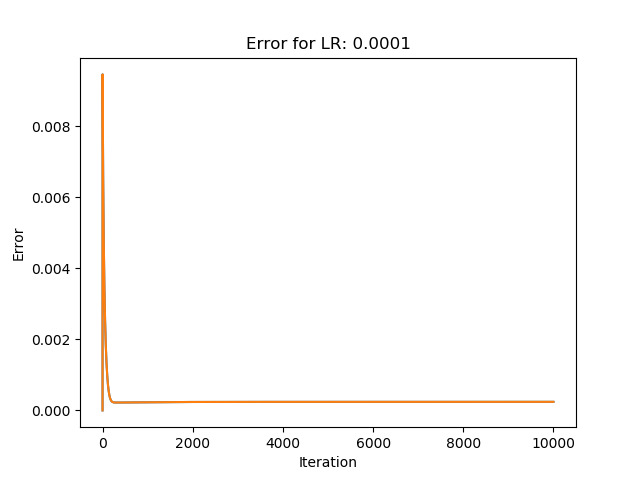
\includegraphics[width=12cm, scale=0.5]{00001.jpg}
	\caption{Best Learning Rate was 0.0001}
	\label{fig:LR_00001}
\end{figure}


%----------------------------------------------

\begin{question}{Gradient Descent Variants}{5}
Throughout this class we have seen that gradient descent is one of the most used optimization techniques in Machine Learning. This question asks you to deepen the topic by conducting some research by yourself.

\textbf{1)} There are several variants of gradient descent, namely \emph{batch, stochastic} and \emph{mini-batch}. Each variant differs in how much data we use to compute the gradient of the objective function. 
Discuss the differences among them, pointing out pros and cons of each one.

\textbf{2)} Many gradient descent optimization algorithms use the so-called \emph{momentum} to improve convergence. What is it? Is it always useful?

\begin{answer}



\textbf{Batch gradient descent} in machine Learning calculates the gradient using the whole dataset. For this the computer needs to have the whole dataset in memory, which is not always doable. Because of that, its also very time consuming. It converts against the global Minimum of konvex functions and local Minimums of non konvex functions.

\textbf{Stochastic gradient descent} calculates the gradient for a single traingingexample. Because of this stochastic gradient descent learns a lot faster than batch gradient descent, however its variance is very high, resulting in highly fluctuating costfunction.


\textbf{Mini-batch gradient descent} can be seen as an combination between stocahstic gradient descent and batch gradient descent, using mini-batches containing $n$ training examples. This results in reduced variance and more stable conversion rate. When mini-batch gradient descent is calculated on gpus, it is possible to reduce the workload by using matrix operations.


\textbf{Momentum} is often used to help the gradient descent algorithm to find the global Minimum. 

Without Momentum there is a high possibility, that GD starts oscillating around a local minimum. In order to reach the global Minimum, this local one needs to be "jumped over". This can be interpeted as a physical impulsive giving a downhill rolling sphere an impuls of energy, to help it overcome obstacles. This "impuls" is usually calculated by looking at the last gradient and adding a part of it to the current gradient. This means, that if the last update to our parameters was big, we guess that the next one will be big, too.
\end{answer}

\begin{figure}[h!]
	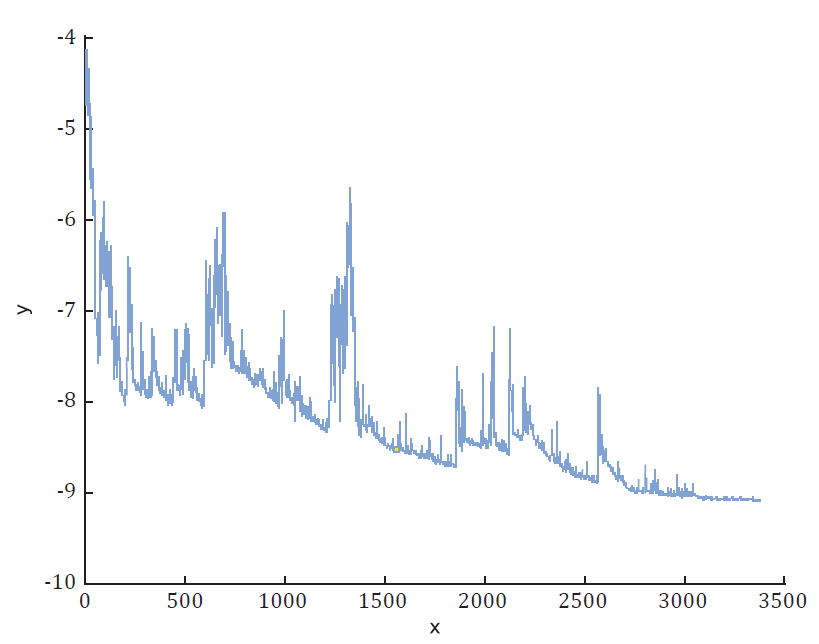
\includegraphics[width=12cm, scale=0.5]{SGD.png}
	\caption{Example for fluctuating cost function for a Neural Network when using SGD [Source: Me]}
	\label{fig:SGD_cost_function}
\end{figure}
\begin{figure}[h!]
	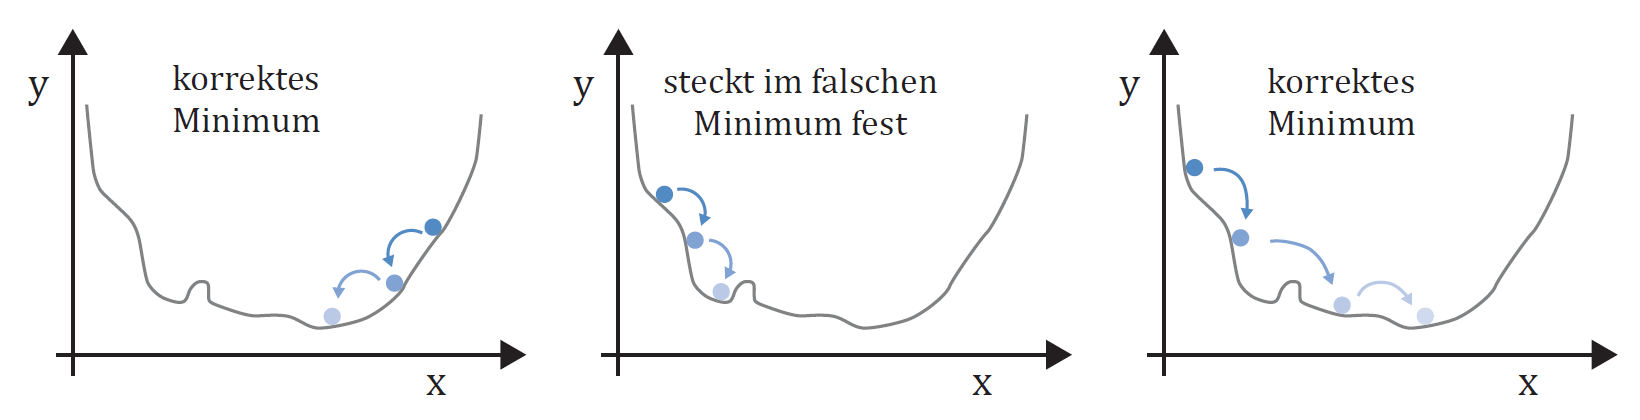
\includegraphics[width=\linewidth, scale=0.5]{momentum.png}
	\caption{Physically interpretation of Momentum [Source: Me]}
	\label{fig:Momentum}
\end{figure}


\end{question}
%----------------------------------------------

\begin{question}[bonus]{Natural Gradient}{10}
Let $\theta \in \mathbb{R}^n$ be a parameter vector
and $J \colon \mathbb{R}^n \to \mathbb{R}$ a cost function.
The negative gradient $-\nabla J(\theta)$ is sometimes called
the \emph{steepest descent direction}. But is it really?
To be able to claim that it is \emph{the} steepest descent direction,
we should compare it to other descent directions
and pinpoint what is so unique about the negative gradient direction.

\textbf{Covariant gradient.}
A fair way to compare descent directions is to make
a small step of fixed length, say $\varepsilon$,
in every direction~$\Delta \theta$ and check
which direction leads to the greatest decrease in $J(\theta)$.
Since we assume that the step size is small, we can evaluate
the decrease in $J(\theta)$ using its first-order Taylor approximation
\begin{equation*}
  J(\theta + \Delta \theta) - J(\theta) \approx
  \nabla J(\theta)^T \Delta \theta.
\end{equation*}
To make precise what we mean by \textit{small} step size,
we need to introduce a norm (or a distance)
in the space of parameters $\theta$.
A good choice, that among other advantages captures the intuition
that some parameters may influence the objective function more
than others,
is the generic quadratic norm
\begin{equation*}
  \norm{\Delta \theta}^2 =
  \frac{1}{2}\Delta \theta^T F(\theta) \Delta \theta
\end{equation*}
with a positive-definite matrix $F(\theta)$;
note that in general $F$ may depend on $\theta$.

\textbf{1)} Find the direction $\Delta \theta$ that yields
the largest decrease in the linear approximation of $J(\theta)$
for a fixed step size~$\varepsilon$.
Does this direction coincide with $-\nabla J(\theta)$?
The direction that you found is known as the
negative covariant gradient direction.

\textbf{Natural gradient.}
In statistical models, parameter vector $\theta$ often
contains parameters of a probability density function $p(x; \theta)$
(for example, mean and covariance of a Gaussian density);
thus, the cost function $J$ depends on~$\theta$ indirectly
through $p(x; \theta)$.
This two-level structure gives a strong hint to what matrix $F$
to pick for measuring the distance in the parameter space
in the most \textit{natural} way.
Namely, one can carry over the notion of `distance' between
probability distributions $p(x; \theta + \Delta \theta)$
and $p(x; \theta)$ (which is known from information theory
to be well captured by the Kullback-Leibler divergence)
to the distance between the corresponding parameter vectors
$\theta + \Delta \theta$ and $\theta$.

\textbf{2)} Obtain the quadratic Taylor approximation
of the KL divergence
from $p(x; \theta)$ to $p(x; \theta + \Delta \theta)$ in the form
\begin{equation*}
  KL(p(x; \theta + \Delta \theta) || p(x; \theta)) \approx
  \frac{1}{2}\Delta \theta^T F(\theta) \Delta \theta.
\end{equation*}
Covariant gradient with the matrix $F(\theta)$ that you found
is known as the natural gradient.

\begin{answer}\end{answer}

\end{question}



%----------------------------------------------

\end{questions}
